% !TeX spellcheck = en_GB
% !TeX root = Report.tex
\phantomsection
\addcontentsline{toc}{section}{Section 1 - Invited Talks}
\sect{Section 1 - Invited Talks} \label{Sect1}
%HSL: I have moved this to the intro
%This section contains a reflection on each of the invited talks in the light of the hypothesis of this report. Full notes from the lectures have been recorded in Appendix 4.

%\phantomsection
%\addcontentsline{toc}{subsection}{Domino Printing Sciences PLC}

\phantomsection
\addcontentsline{toc}{subsection}{Imagination Technologies}
\subsect{Lecture 1}

\lipsum[2]
 



%\phantomsection
%\addcontentsline{toc}{subsection}{ARM}

% !TeX spellcheck = en_GB
% !TeX root = Report.tex
\phantomsection
\addcontentsline{toc}{subsection}{David Parker - Southampton Photonics}
\subsect{Lecture 2 -  David Parker \& Perpetuum}


%\inote{Give a brief intro to them}
Perpetuum are a Southampton based business specialising in energy harvesting modules. 
They were founded in 2004 and they began life as a component supplier for their power module.
\todo[color=red]{Needed?}Perpetuum do not classify as an emerging company in the current day, but the early life of the company and their patent acquisitions are discussed here. 
They are a venture capital funded start-up involving multiple companies.
It was a spin off from a technology developed at Southampton University. 
%\inote{Show Perpetuum is a start up.}

%\inote{Discuss patent acquisitions of Perpetuum}
%http://patents.justia.com/assignee/perpetuum-ltd?page=2
Perpetuum currently hold 22 patents to date. 
Their first was issued on the 23rd August, 2007, some 3 years after they began.
These initial patents prevented any other businesses from being able to reproduce their technology. 
However, the company initially struggled with business.
Their target market was the Oil and Gas industry as they use large drills which vibrate, making it a perfect spot to house their module.
The main issue was that the target market had no application for the module that Perpetuum were attempting to supply. \todo{find out what exactly they were initially supplying}

%In 20xx \todo{find when Parker joined}, David Parker was asked to join Perpetuum. 
Due to the business not fulfilling their potential, they undertook a change. 
The core competencies of the company were considered.
It was easy to see that the main core competency of Perpetuum was in developing energy harvesting modules. 
A second core competence was added to the company of developing a wireless sensor for their module, transferring the product developed from a component, to a system.
This change in focus was accompanied by a change in market - the system was aimed at the transport industry, particularly trains, where there was a gap for a remote monitoring system of the bearings and suspension. 

Even though Perpetuum had a great, novel idea with patents to protect them, it did not make them money by owning the patents alone.
The patents definitely helped, as it meant no other company could have undermined them during the time they were pursuing the non-existent market in oil and gas.
The patents here acted as a barrier to the market, giving them the time to find the correct opportunity to become a success.
Perpetuum have grown rapidly since the shift in core competence and market, with a turn over of around \pounds 2 million in 2013.
There is no doubt that Perpetuum will become ever more successful through the combination of a good idea in the correct market, with patents to protect their product. 

%Another interesting point raised in the lecture by Dr Parker, was that IP is only effective in hardware industry.
%Software is difficult to patent \todo{why is software difficult to patent? Refer to the introduction on patents}

%\inote{Discuss that even though they had patents, they were in the wrong market.}

%\inote{Now they are in a good market, their patents are protecting them and they are doing well.
%Define ``well''. 
%Are they established yet?}

%\inote{Parker briefly spoke about that software is difficult to patent, but hardware is very effective. 
%Results in us looking at hardware companies rather than software.}


%\phantomsection
%\addcontentsline{toc}{subsection}{Imagination Technologies}


% !TeX root = Report.tex
\phantomsection
\addcontentsline{toc}{subsection}{Lecture 3 - Iain Gavin \& Amazon Web Services: HAILO}
\subsect{Lecture 3 - Iain Gavin \& Amazon Web Services: HAILO}

%\inote{Spell checker is up the creek, all my sections need checking - Will do in Soton}





Amazon is, without any reasonable doubt, an established company. 
Founded by Jeff Bezos in 1994 as an online bookshop the company shipped their first book in July 1995~\cite{seattle}. 
The company now has three different parallel business interests. 
The original retail aspect, a 3$^{rd}$ party selling service via the website and Amazon Web Services (AWS).
AWS powers the other two aspects of the business by providing the IT infrastructure that enables such excellent customer service but also acts as an accelerator for other businesses by removing the requirement for on-premises IT solutions. 
They achieve this by maintaining large sever farms from which computing power can be \emph{rented} to facilitate the IT needs of a company. 
They also provide varying degrees of cloud based storage; subject to access latency.

AWS considers a typical split in effort toward a computing heavy business venture, with an on-premises IT solution, to be $30\%$ towards the actual business and $70\%$ towards IT overheads~\cite{gavin2014ams}. 
Their goal is to reverse this distribution by providing the infrastructure for the business. 
One such company that has succeeded using AWS is HAILO~\cite{gavin2014ams}. 
Launched in $2011$ with investments totalling over \$$80$ million from some well known sources such as Union Square Ventures, Accel Partners and Sir Richard Branson~\cite{hailo}.
The company maintains a smartphone app that links customers with the local taxi services however this idea is not unique. 
At the time there was already a large market for smartphone enabled cab rides so something else must have been their source of success~\cite{ventureBeat}. 
Market saturation and a software only product makes patenting redundant so it must have been down to the delivering and quality of the service that has made them a global success. 
Disassociating IT from the business using AWS may well have been a contributing factor to HAILO's ability to concentrate on product delivery.


The Amazon group as whole is very technology driven, the founder filed the first two patents under ``Amazon.Com, Inc'' just before their first sale, and considers innovations as the best method to drive down the prices of the products they sell~\cite{bezos1998secure1,bezos1998secure2}. 
Reasoning behind this idea is shown in Figure~\ref{fig:ScaleInnovation}.
This cycle enables price reduction which naturally improves sales. 
The key step is providing the technology which can improve efficiency therefore staying ahead of competitors. 
Amazon keeps delivering the required technology, patenting aggressively, and at the end of $2013$ created another media buzz by publishing a patent for ``anticipatory package shippin''~\cite{spiegel2013method}!



%\inote{Need to sexify}


\begin{figure}
	\centering
	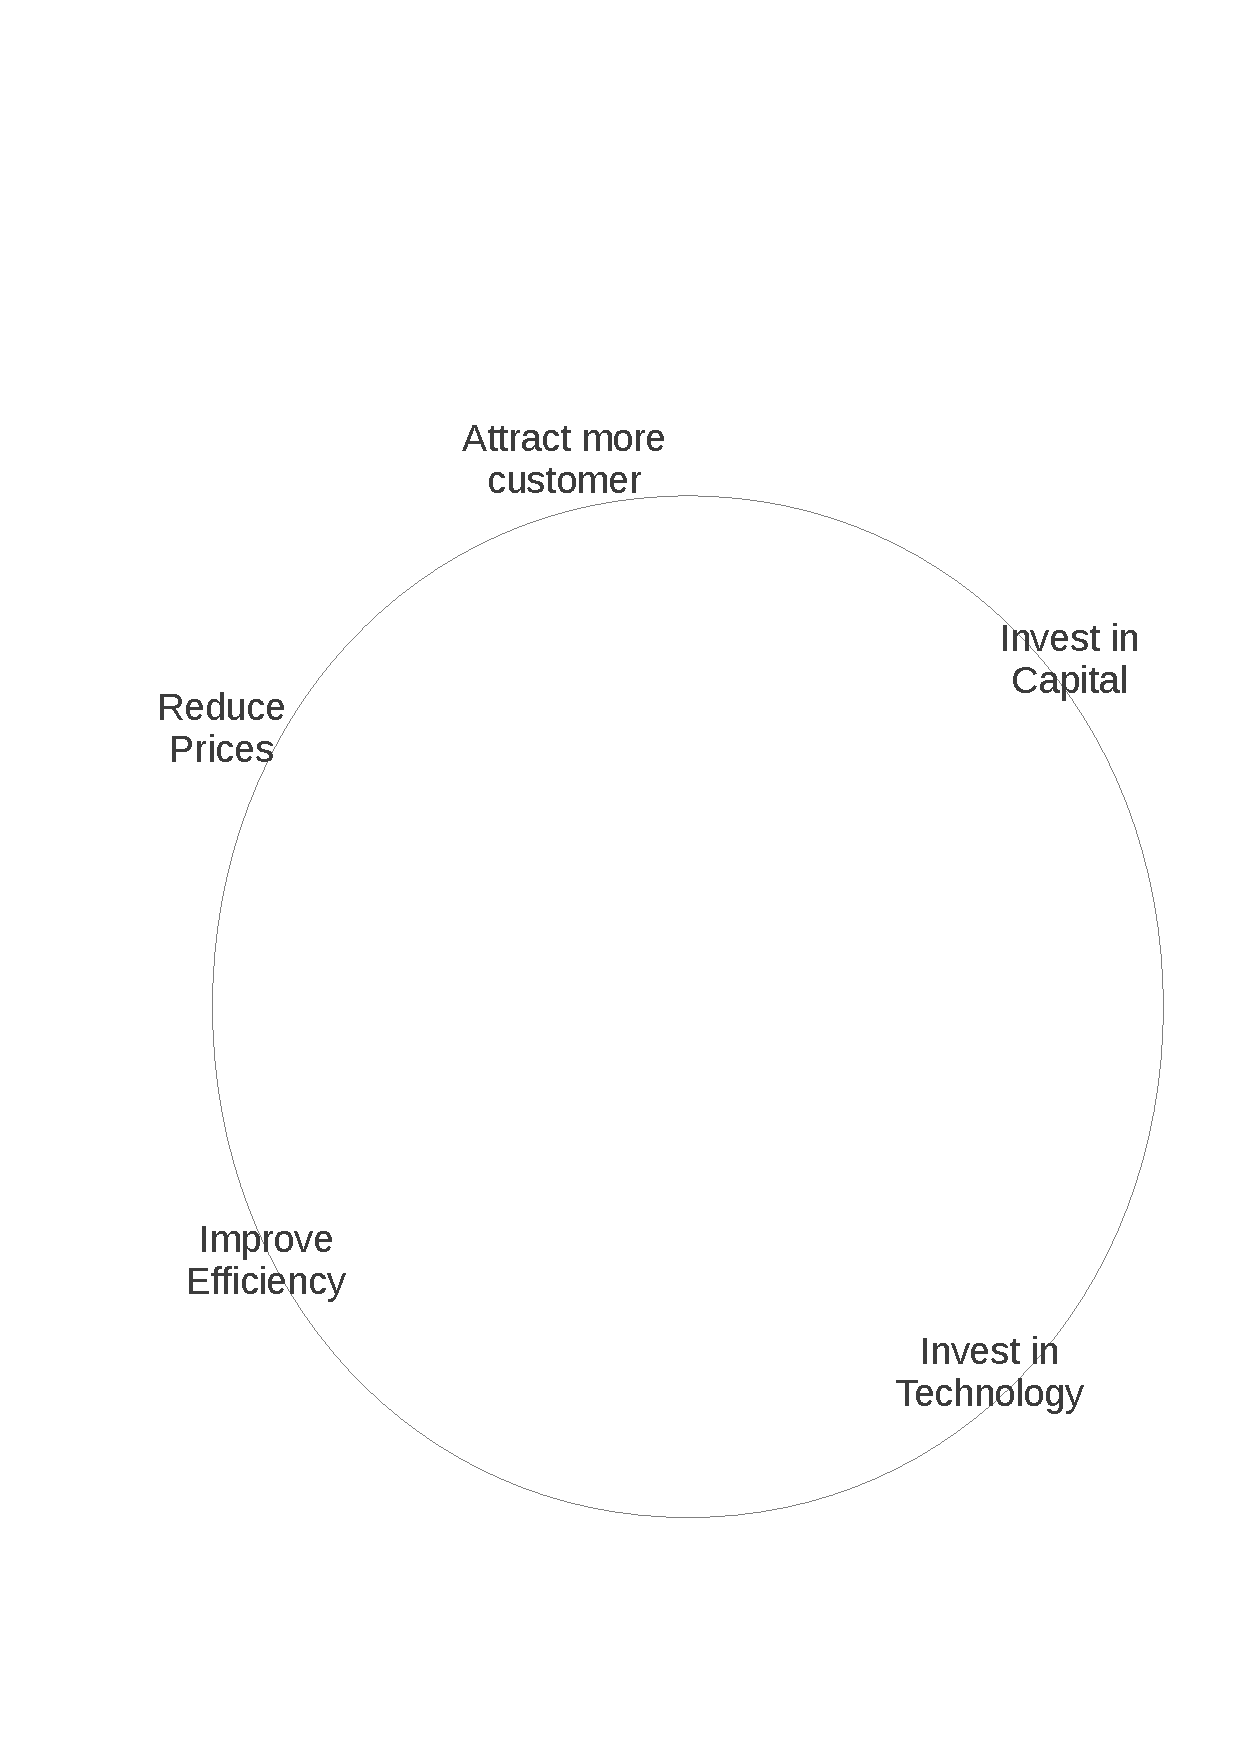
\includegraphics[width=0.4\textwidth]{./Figures/ScaleInnovation.pdf}
	\caption{Scale \& Innovation Drives Down Costs. Taken from~\cite{gavin2014ams}.}
	\label{fig:ScaleInnovation}
\end{figure}



\phantomsection
\addcontentsline{toc}{subsection}{Reflections}
\subsect{Reflection on Common Themes}
\inote{Reflection on Common Themes - HSL I don't think this is needed. We're running out of words and I do summarise all companies in the conclusion. Thoughts?}



